\chapter{Architectural design}

\section{Overview}
This chapter describes the different components of PowerEnjoy and how they interact with each other, starting from an high level view of the system and finally explaining in detail the sub-components.

\section{High level components and their interaction}
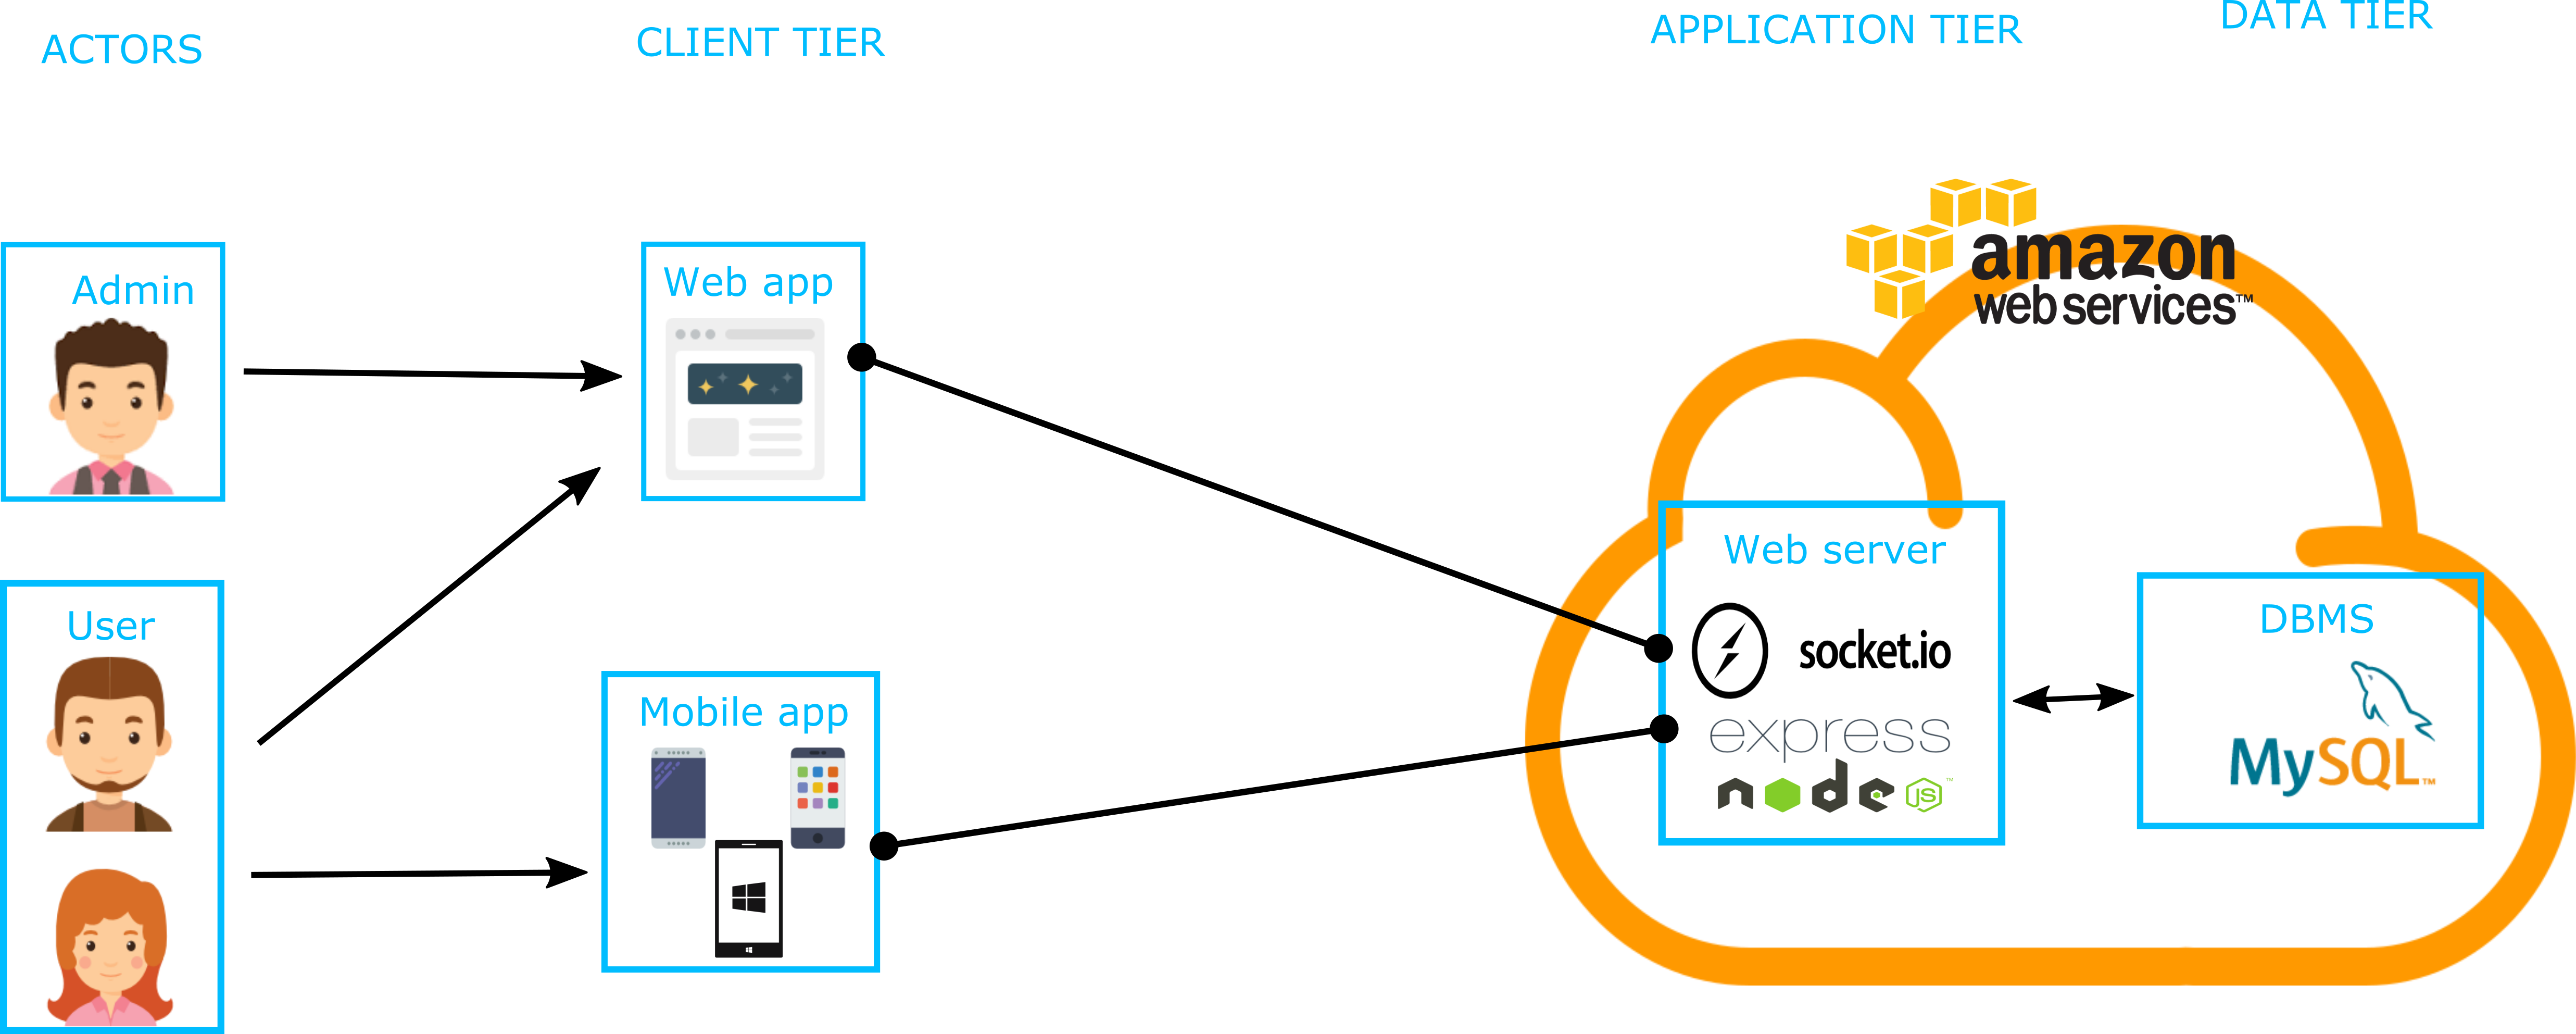
\includegraphics[width=\textwidth, keepaspectratio]{../images/architectural_design/high_level_view.png}

PowerEnjoy is composed by three main components: DBMS, web server and client application.
These can be mapped to three tiers in a three-tiers architecture: the data tier is the DBMS, the application tier is the web server and the GUI tier is the client application.
The client application provides the UI through which the users can access the service offered by PowerEnjoy.

The UI makes requests to the web server that is in charge of elaborating those and eventually of providing a valid response.
The client application is waiting for events from the web server and it updates the UI according to the data received.

The web server, while is processing the requests, can make call to external API and query the database.

\section{Component view}

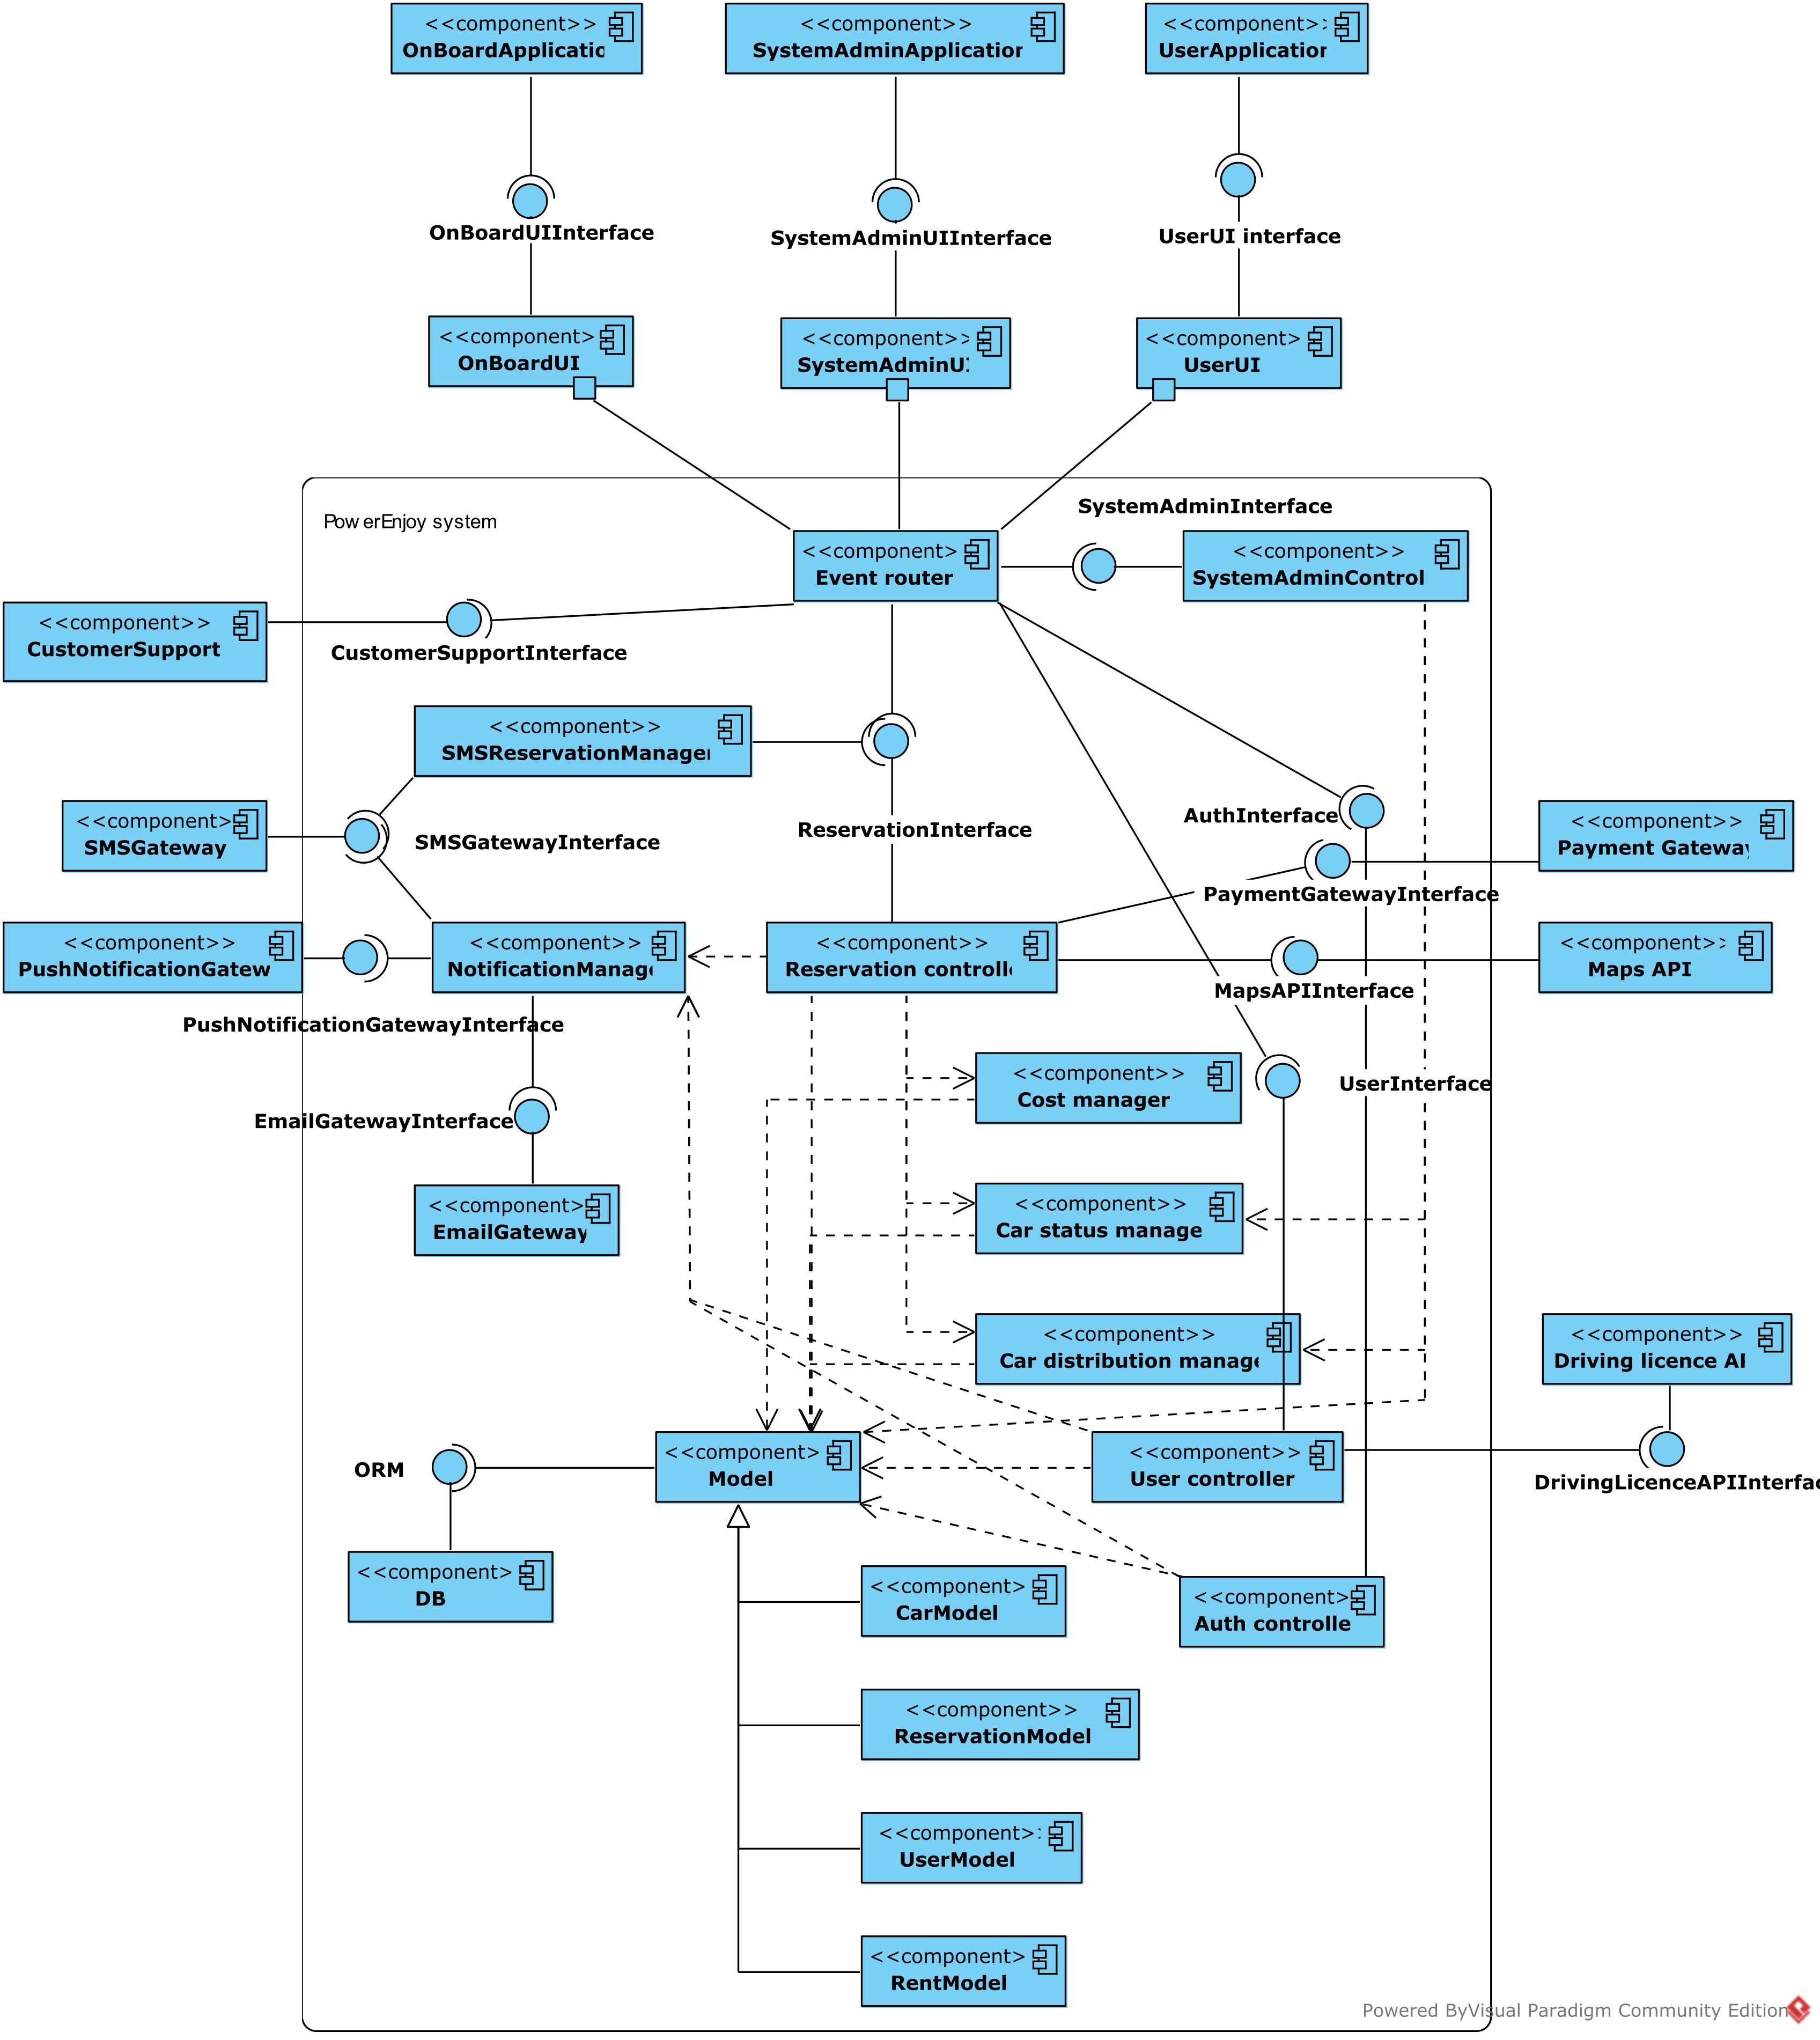
\includegraphics[width=\textwidth, keepaspectratio]{../images/architectural_design/component_diagram.png}

The PowerEnjoy system runs a websocket server, as you can see from the high level view diagram, that receives events from the end-user applications.

The EventRouter dispatches the requests to the appropriate Controller that elaborates the request.
During this operation the controller can use other components of the system or can make calls to external services.

The ReservationController is the main controller and is in charge of managing all the process that involves a reservation, starting from the submission of a reservation request until the end of the rent.
It can be called by either the EventRouter or the SMSReservationManager.

It uses some internal and external components in order to fulfill all the received requests:
\begin{itemize}
\item it uses an external PushNotificationGateway in order to send real-time push notifications to users’ mobile app.
\item it uses an external SMSGateway in order to send SMS notification to users’ mobile phone.
\item it uses an external PaymentGateway in order to complete a payment after a rent is finished.
\item it uses an external MapsAPI in order to locate users and cars into a map. In addition it uses the navigation API, that are part of the Google Maps API, in order to suggest the right journey to the user in case of ‘save money’ option.
\item it uses the internal DiscountManager in order to calculate the discount to apply at the end of a rent.
\item it uses the internal CarStatusManager and CarDistributionManager in order to check whether a car is available or not.
\end{itemize}

The AccountController is in charge of the process of registration and modification of user’s profile and settings.
It uses an external Driving licence API, provided by the ‘Motorizzazione Civile’, in order to check if a driving licence is valid or not.

The AuthController is in charge of checking the validity of the credentials during the login process.

All the controllers use instances of Model in order to retrieve data from the DB.

\section{Deployment view}
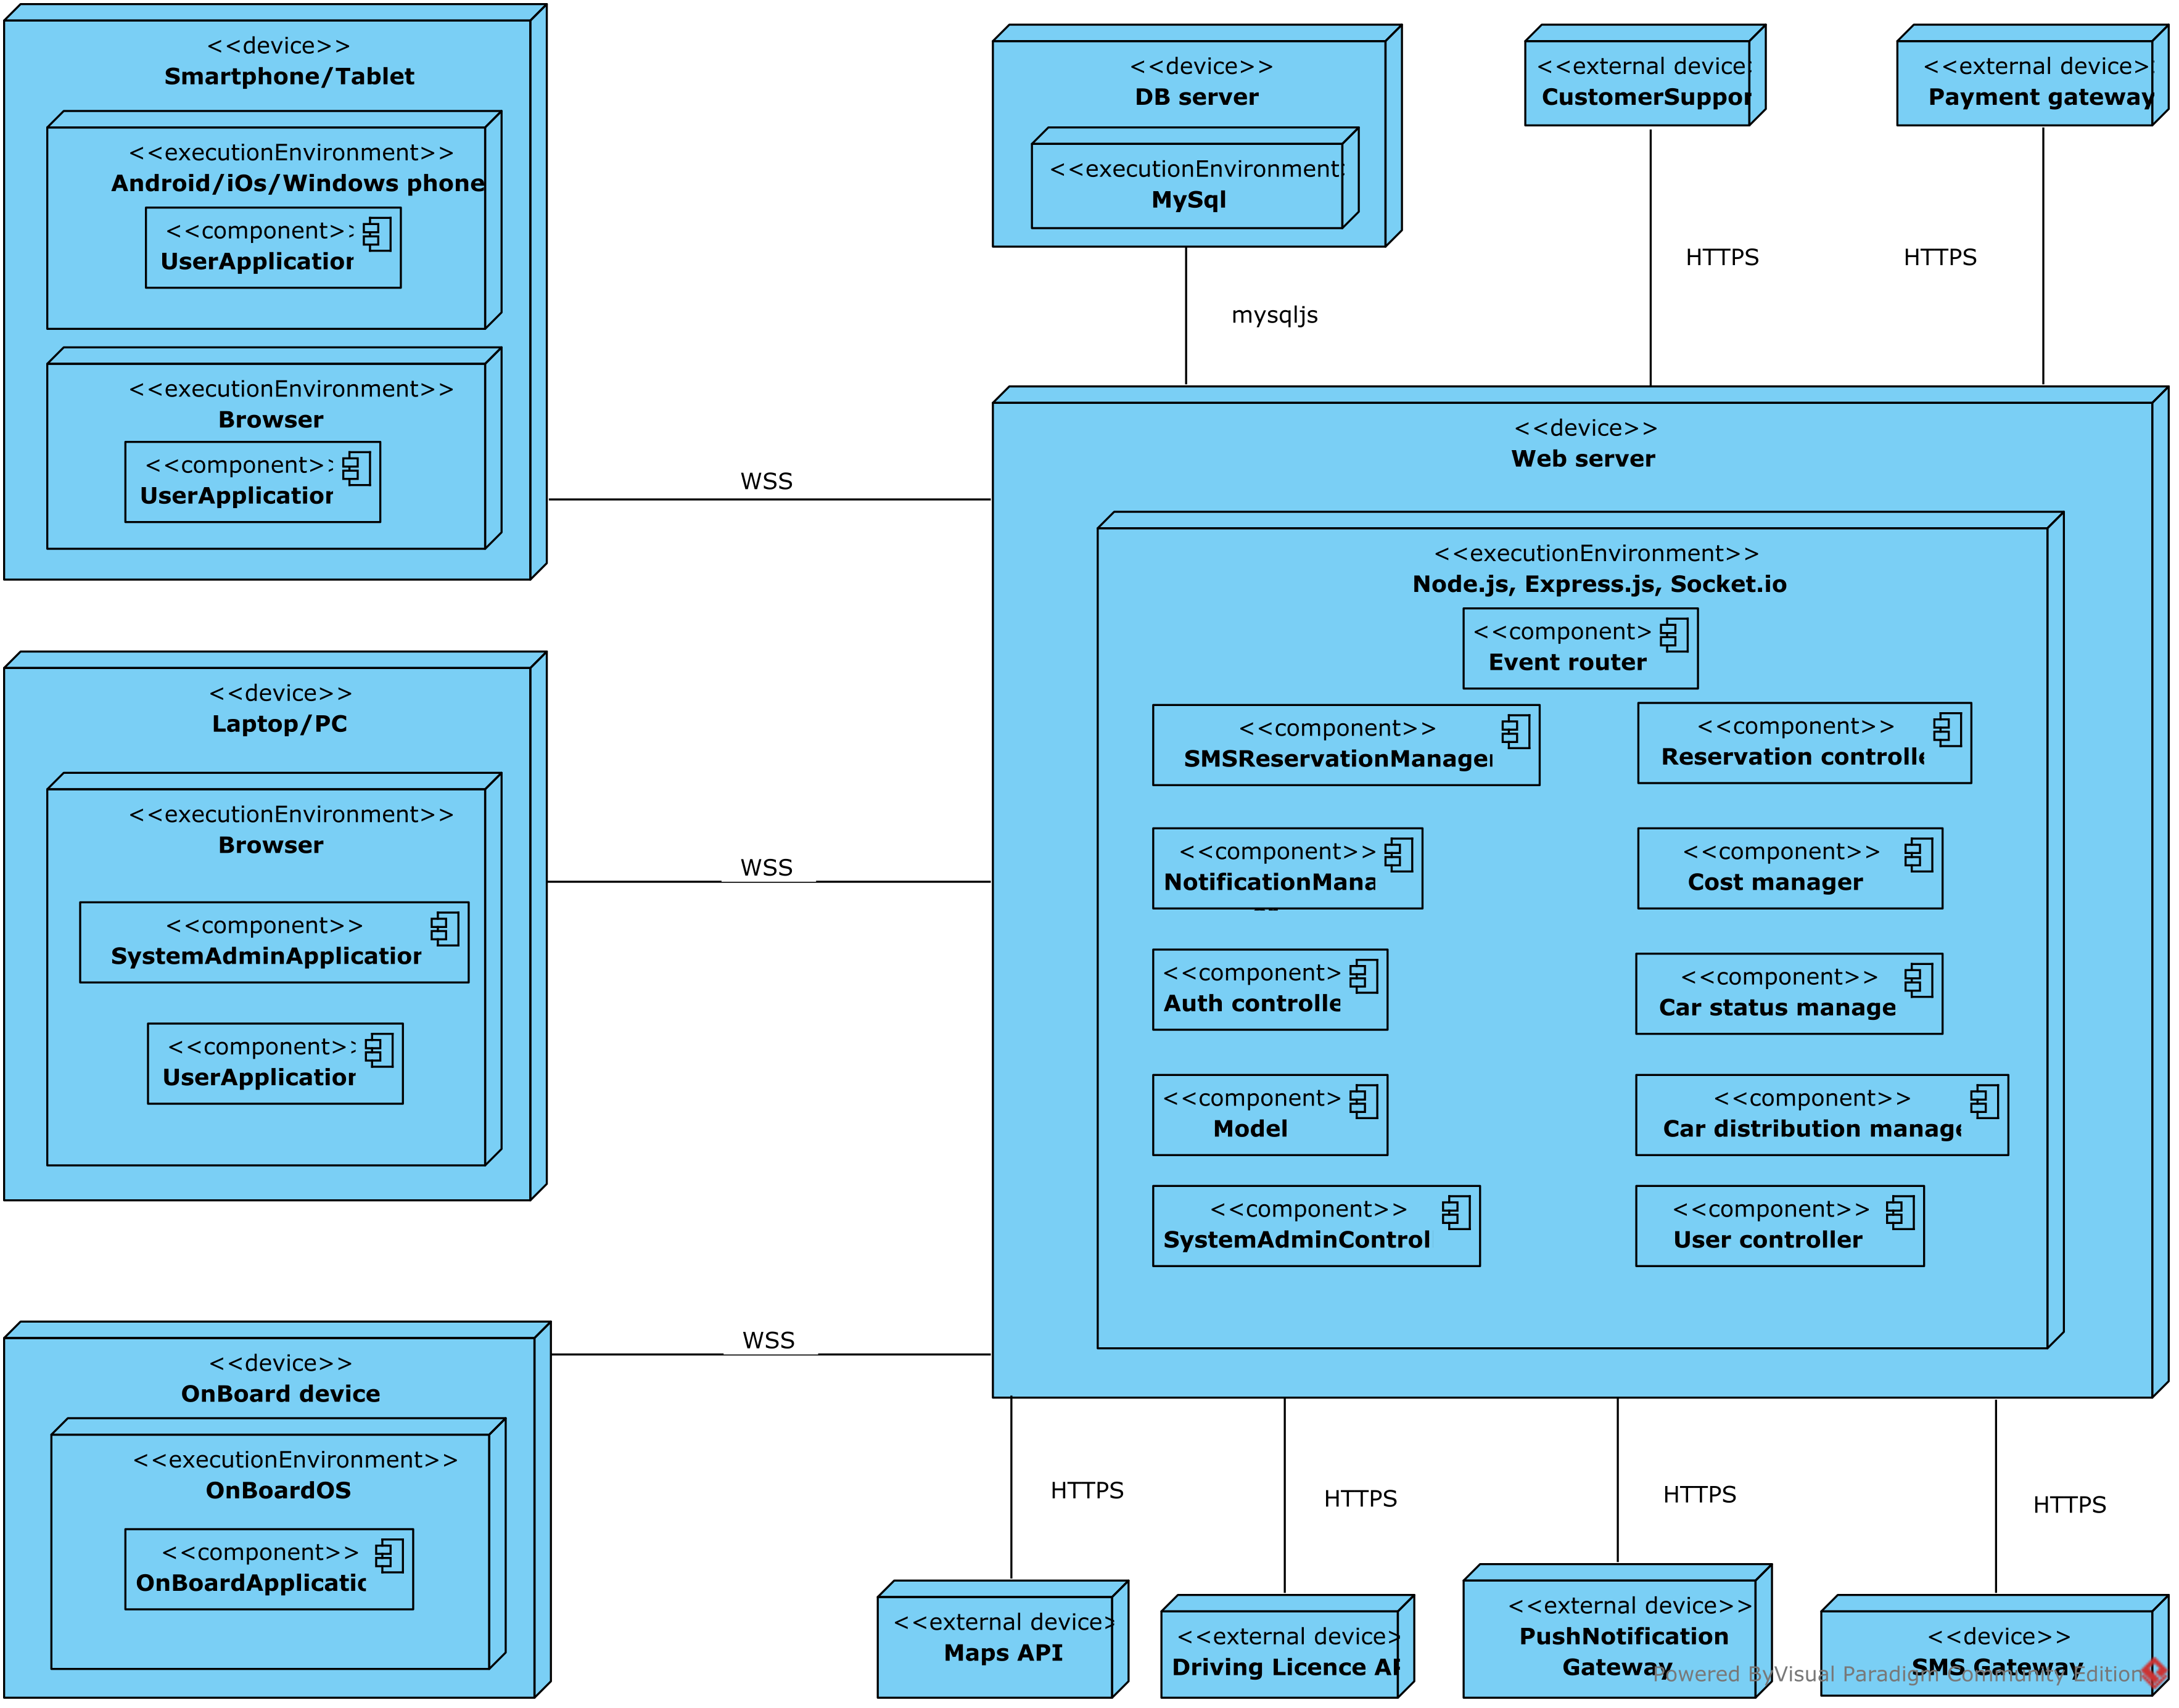
\includegraphics[width=\textwidth, keepaspectratio]{../images/architectural_design/deployment_diagram.png}

In this section the components defined in the previous section are placed within a device.
The following diagram explains where each component is and how  different devices communicate between them.

JSON is used to encapsulate data inside a standard structure and only JSON messages are exchanged between our internal components.
This choice makes easier the exchange of messages, even complex objects, among components built with different technologies.

\section{Runtime view}
In this section are presented some sequence diagrams that explain the interactions among components showed in Component and Deployment diagrams.

\subsection{Login}
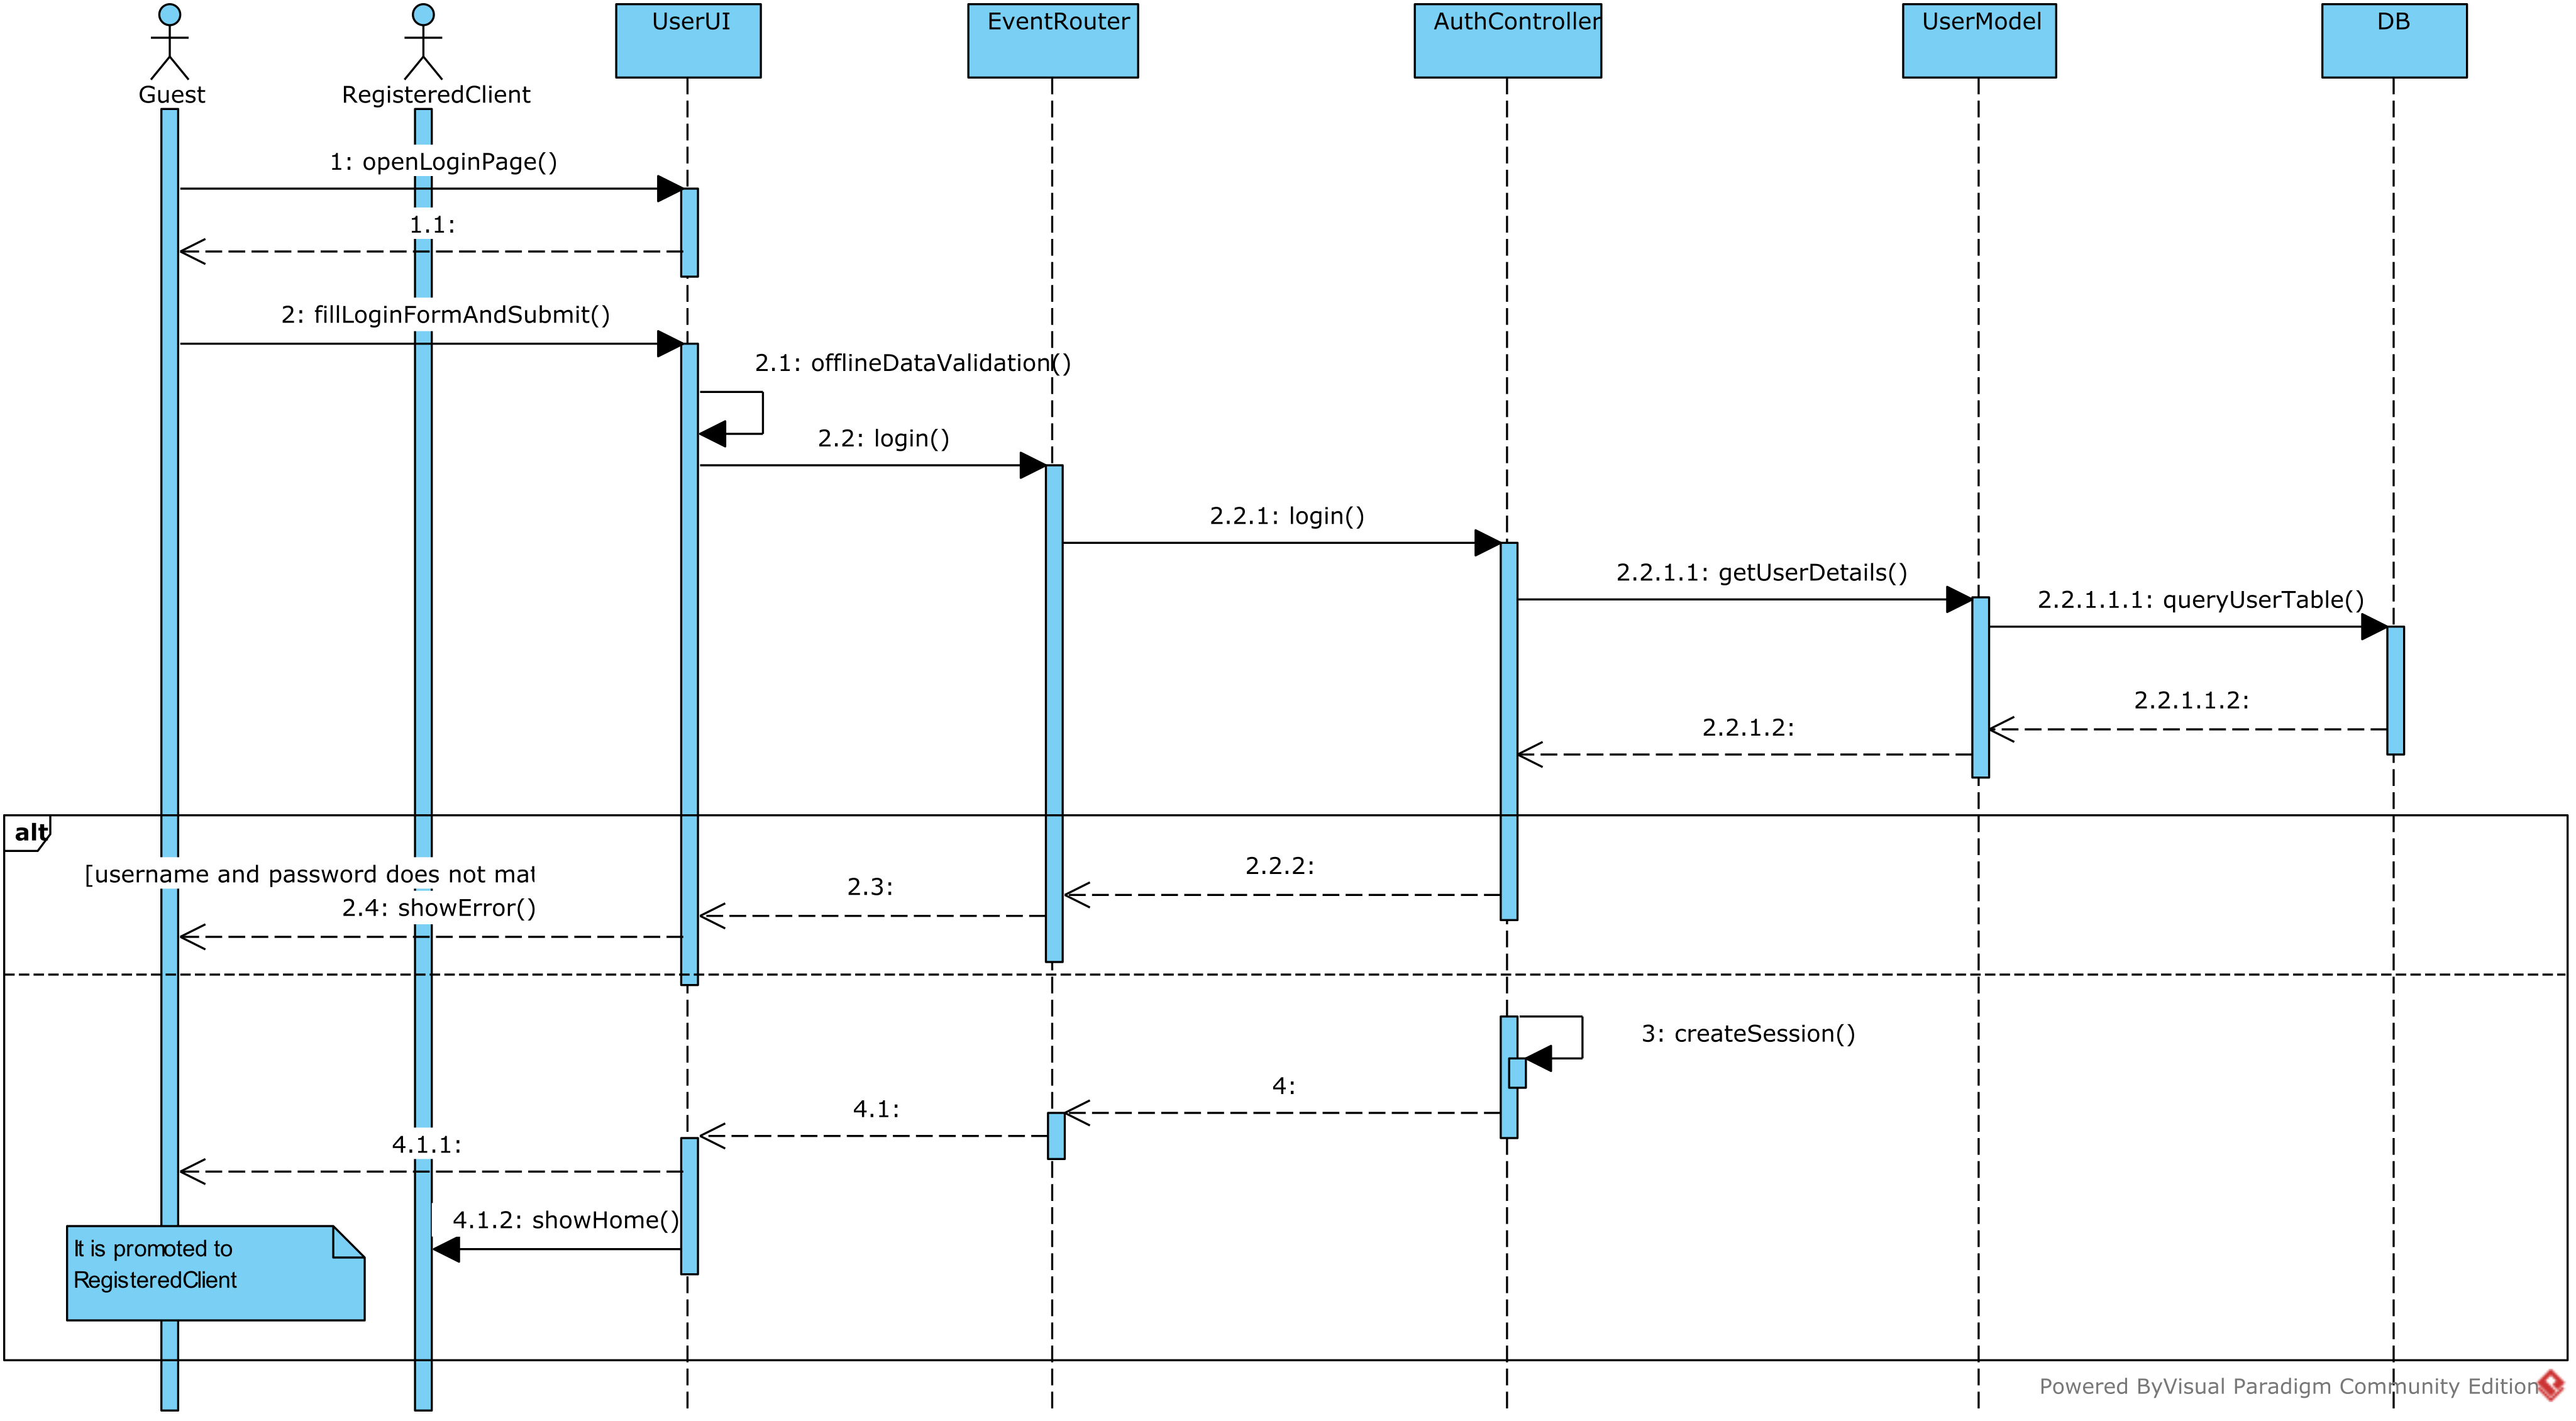
\includegraphics[width=\textwidth, keepaspectratio]{../images/architectural_design/rv_login.png}

\subsection{Reservation through mobile app}
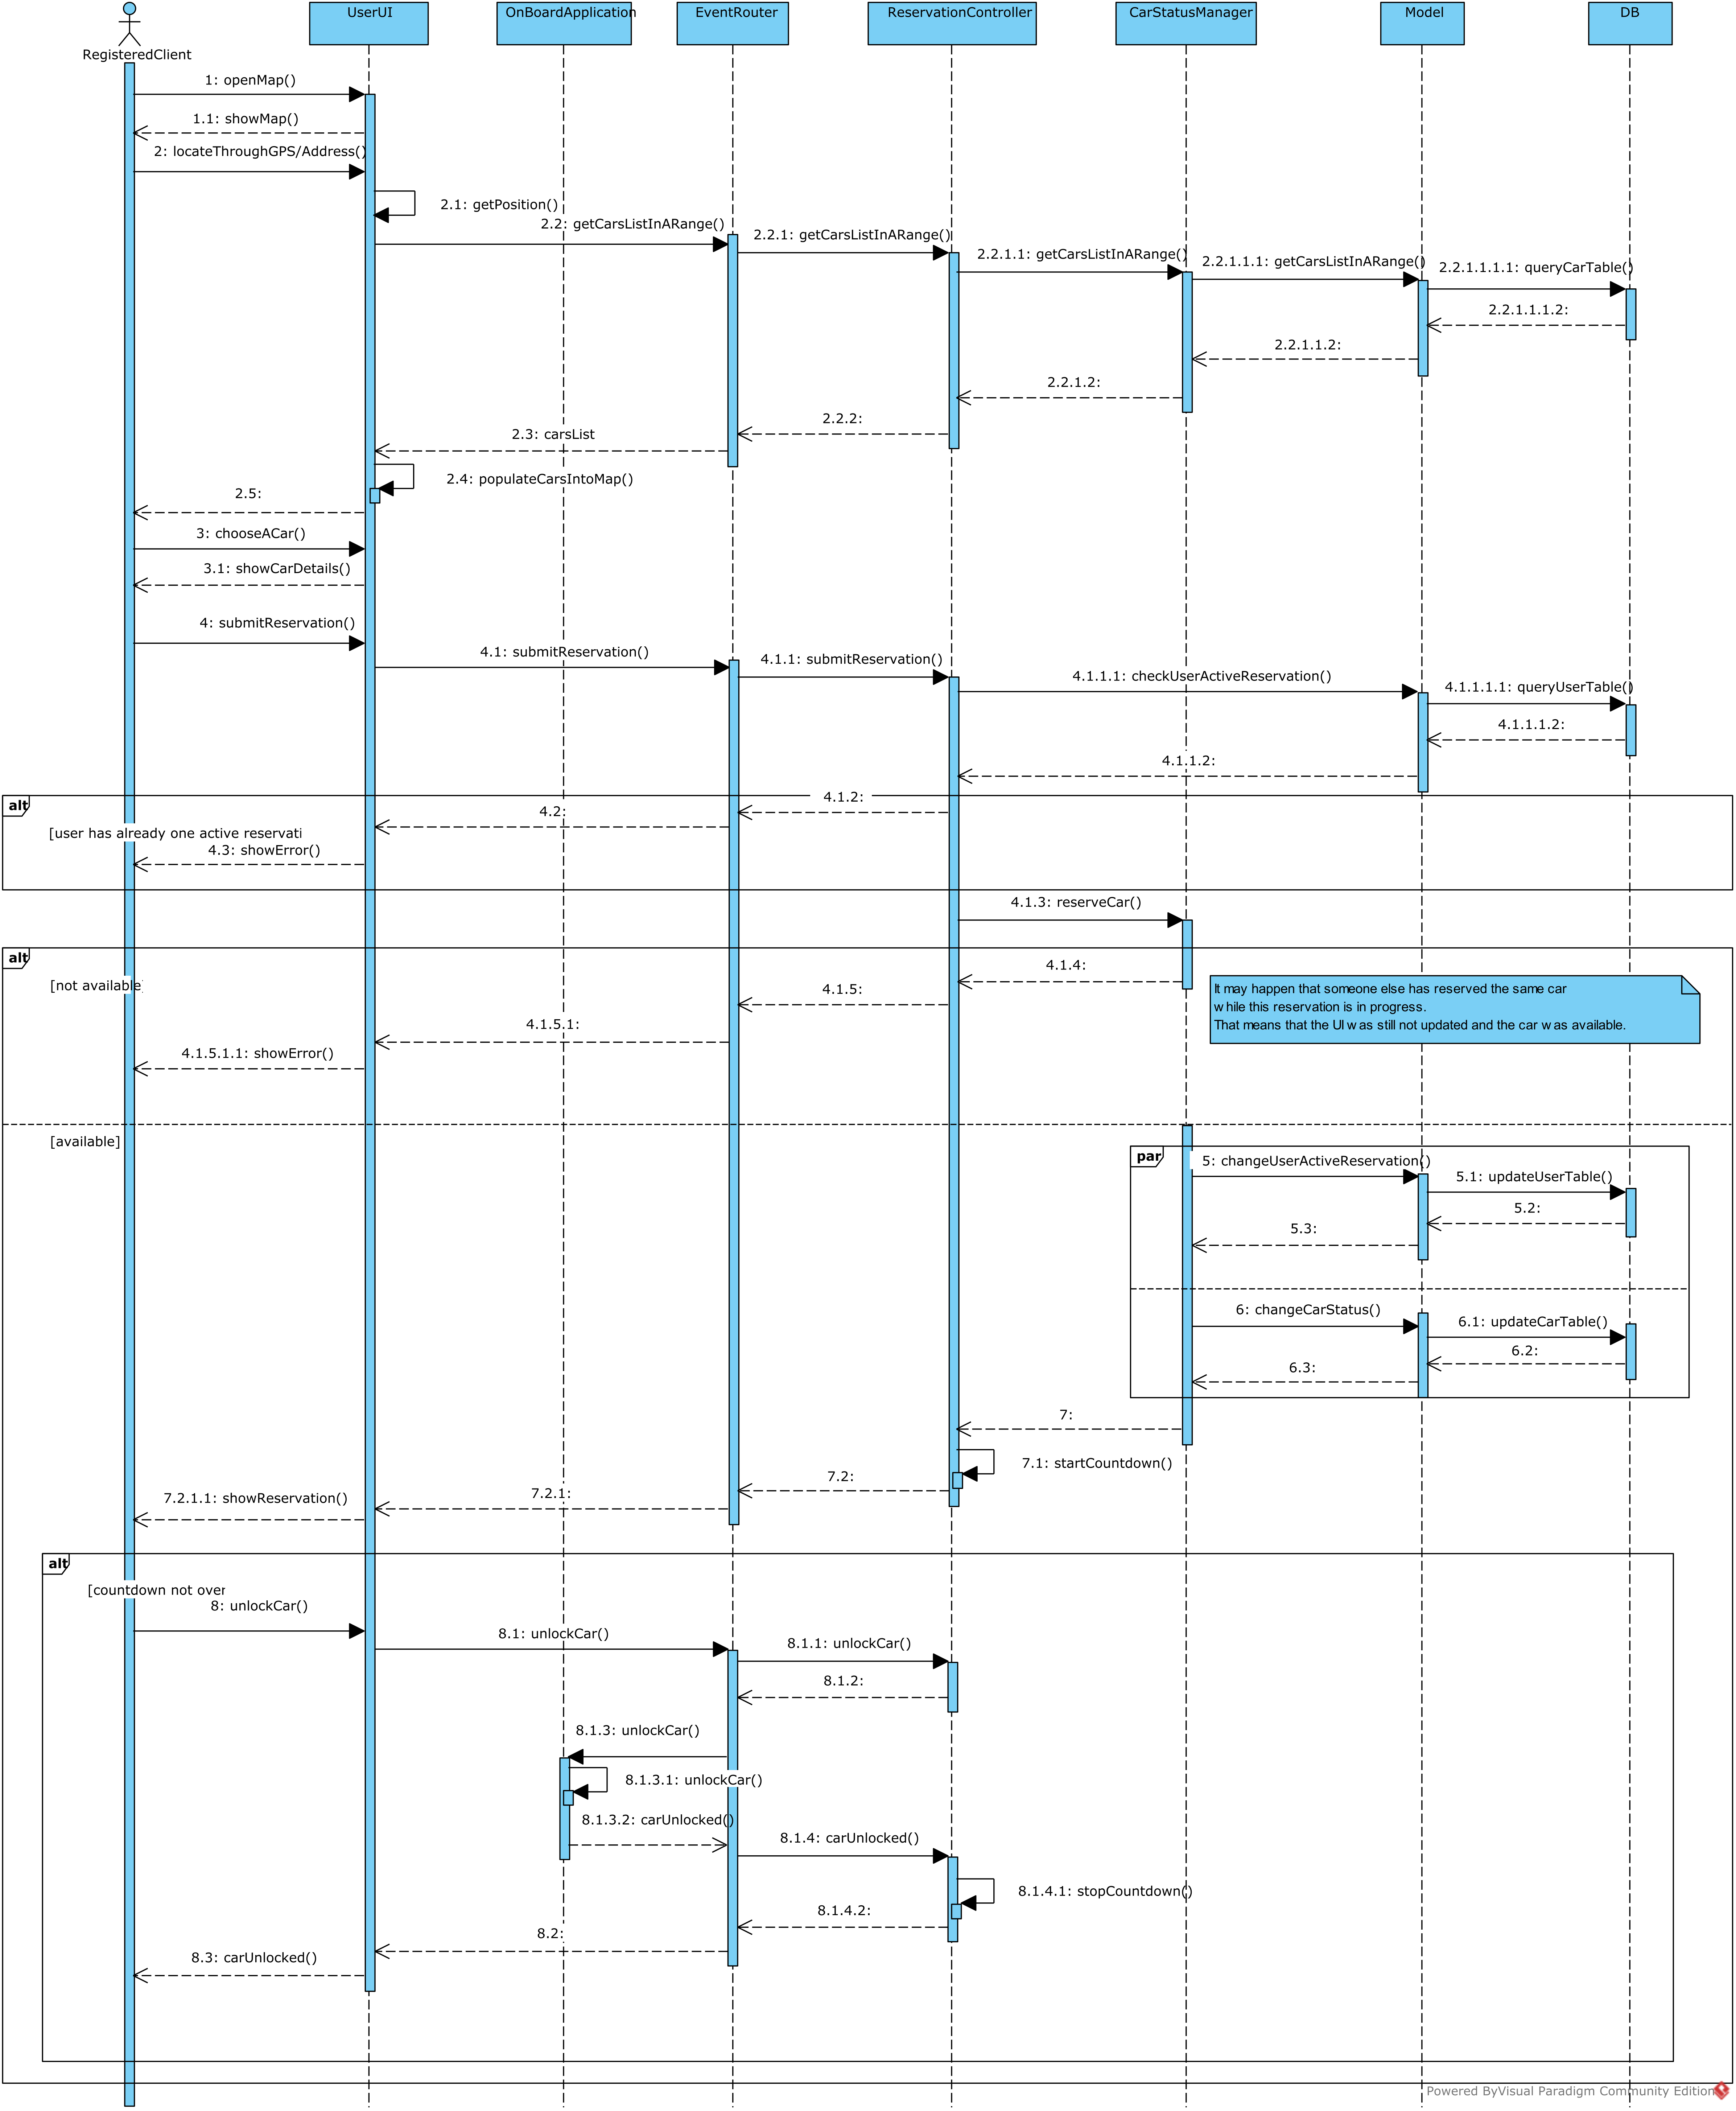
\includegraphics[width=\textwidth, keepaspectratio]{../images/architectural_design/rv_reservation.png}

\subsection{Usage of on board application}
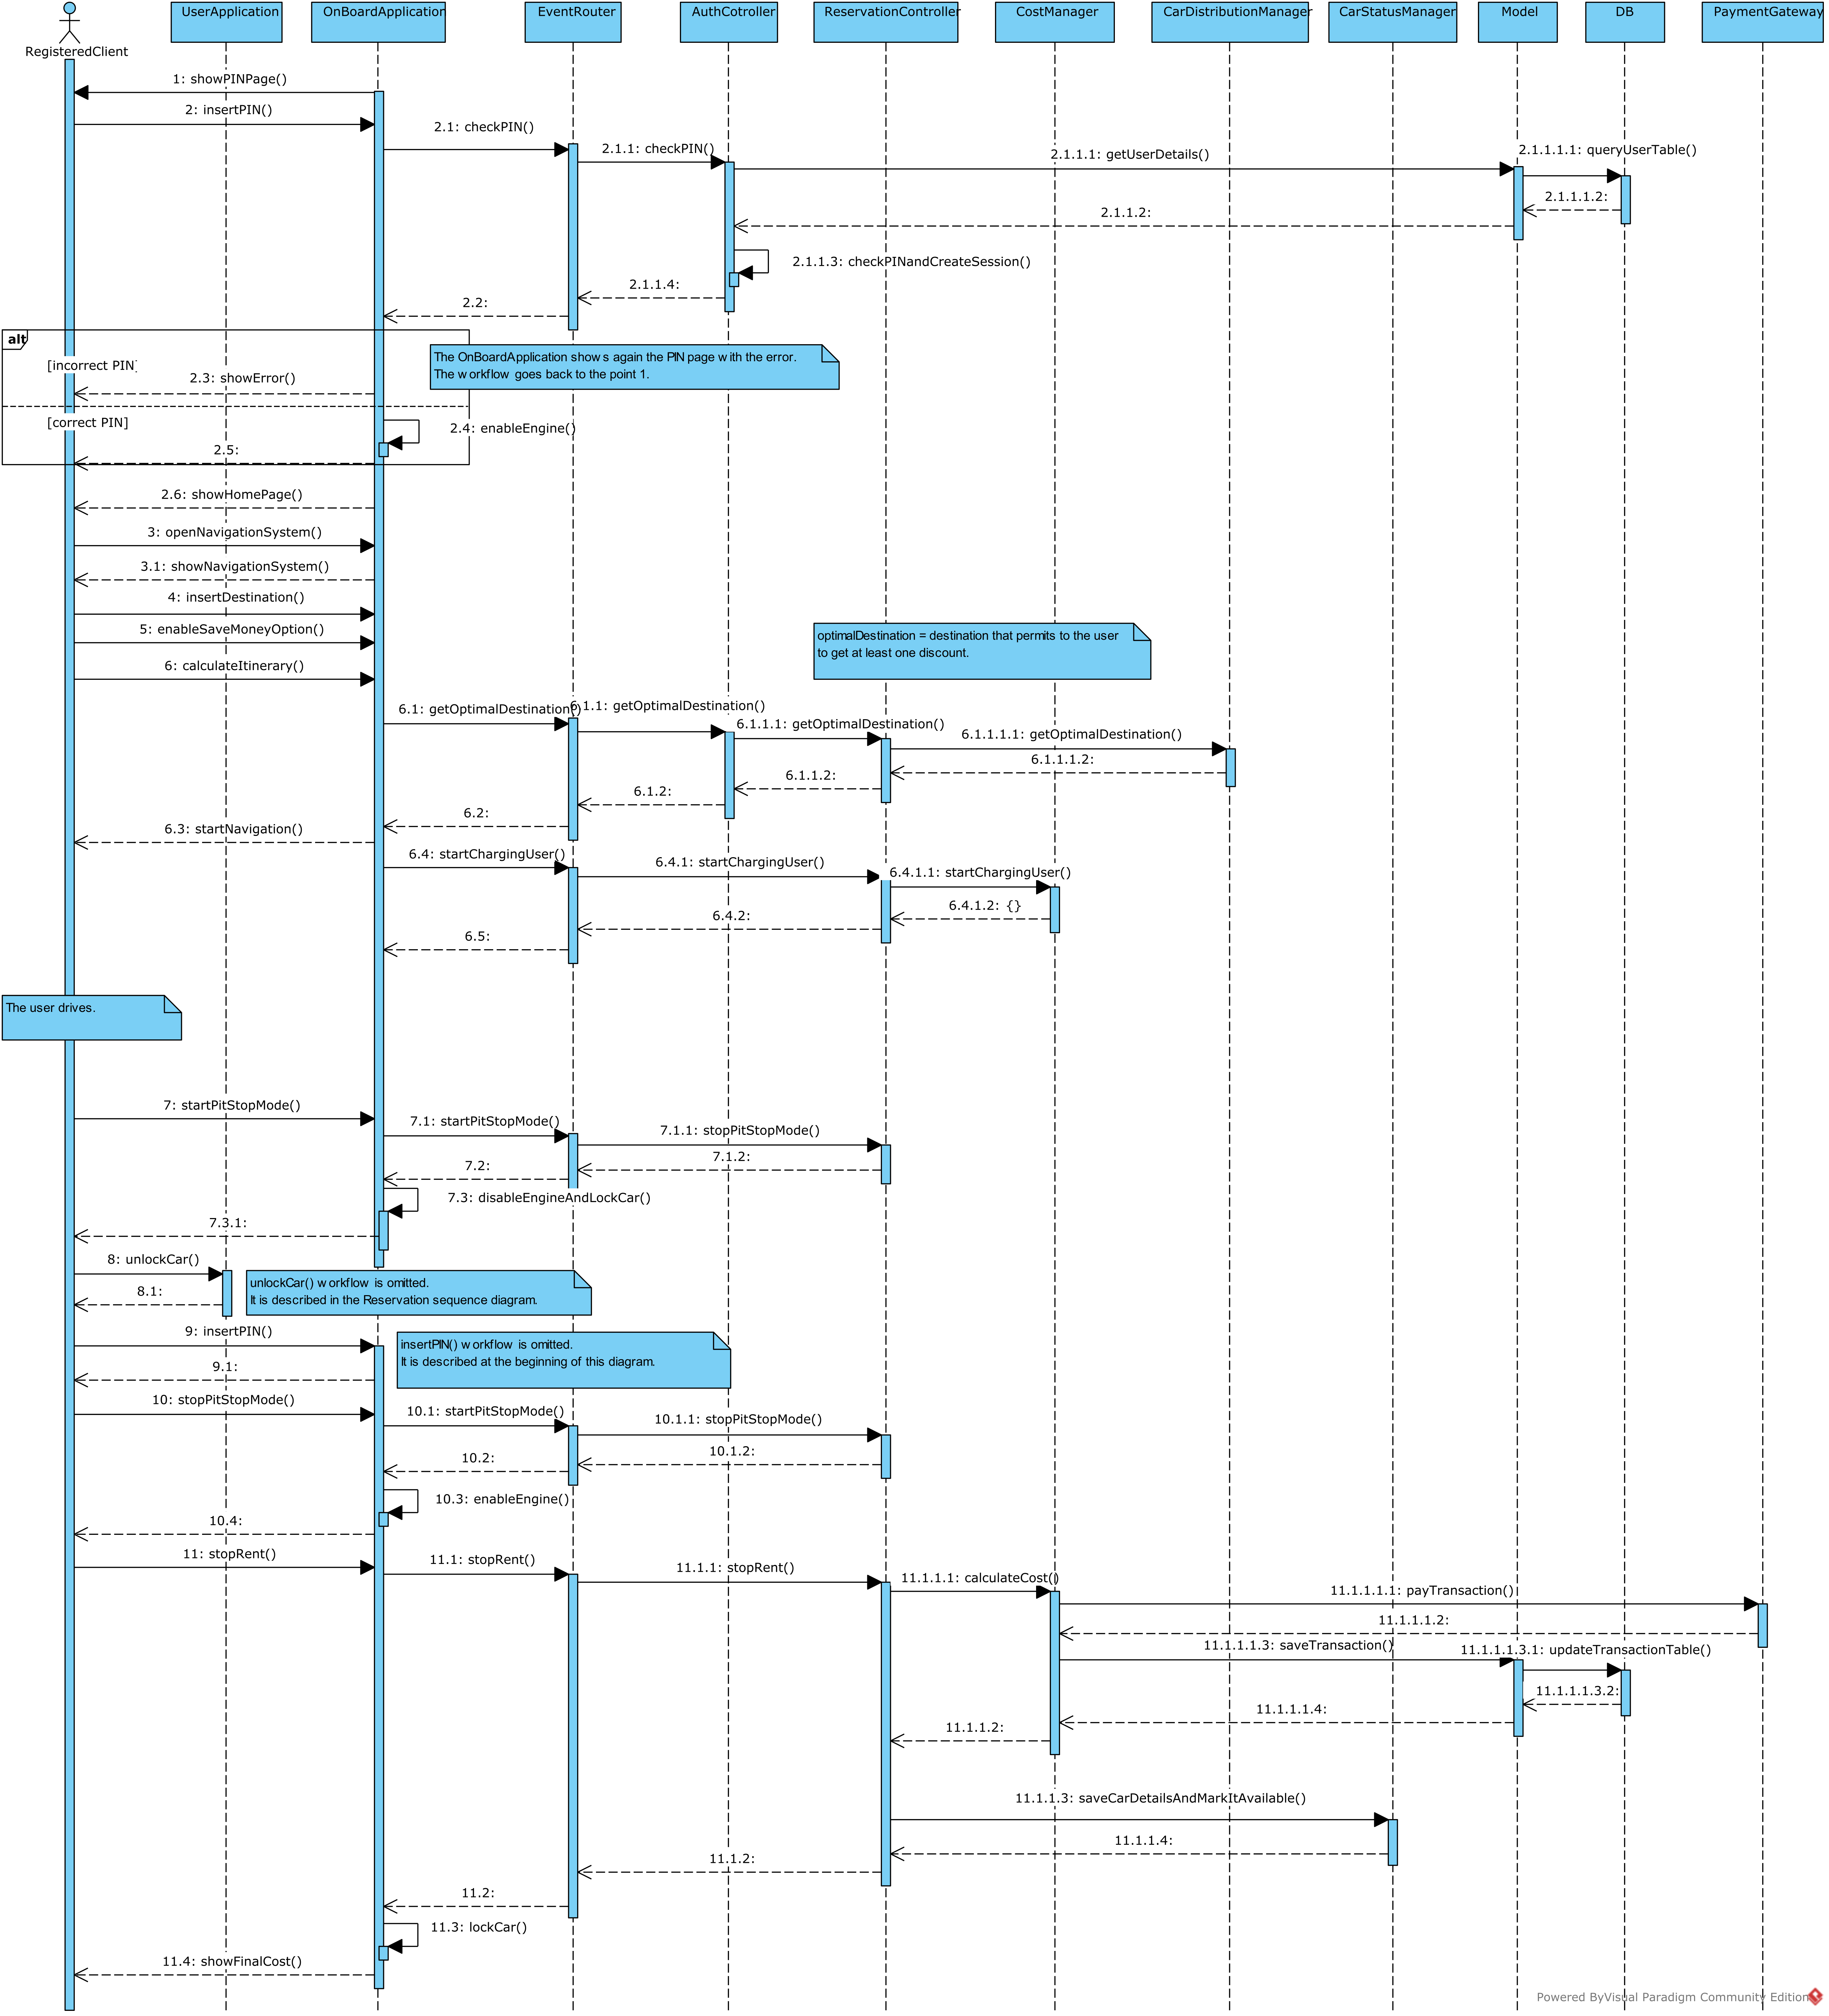
\includegraphics[width=\textwidth, keepaspectratio]{../images/architectural_design/rv_onboard.png}

\section{Component interfaces}
In this section all the interfaces, previously shown in the Component Diagram, are analyzed.

\subsection{UserUI interface}
This interface provides an entry point to the system for Guest users and Registered Clients, through web/mobile application.

The following list contains the main methods provided by this interface:
\begin{itemize}
\item showHome()
\item showLogin()
\item showSingUp()
\item showAccount()
\item showReservationPage()
\item showMap()
\item showCarDetails()
\item submitRegistration()
\item submitLogin()
\item submitReservation()
\end{itemize}

\subsection{SystemAdminUIInterface}
This interface provides an entry point to the system for the System Administratror.

The following list contains the main methods provided by this interface:

\begin{itemize}
\item showHomeAdmin()
\item showAdminLogin()
\item showAdminAccount()
\item showMenu()
\item showDataEditor()
\item submitAdminLogin()
\end{itemize}

\subsection{OnBoardUIInterface}
This interface provides an entry point for Guest users and Registered Clients, through the on board application.

The following list contains the main methods provided by this interface:
\begin{itemize}
\item showEnterPinScreen()
\item showOnBoardHome()
\item showNavigationSystemHome()
\item submitAddress()
\item submitSaveMoneyOption()
\item submitTerminateRent()
\item submitPitStopMode()
\item stopPitStopMode()
\item submitPin()
\item submitAskForHelp()
\end{itemize}

\section{Selected architectural styles and patterns}
This section exposes the architectural decisions for the development the system of Power Enjoy and the reasons related to each choice.

\subsection{Overall architecture}
\subsubsection{Service Oriented Architecture}
SOA fits perfectly the needs of  the system of Power Enjoy, starting from the calls to external services to the communication between the different parts of the data and business models, the involved devices and each architectural layer.

\subsubsection{Client - server architecture}
PowerEnJoy is an on-demand service usable by the client through website, smartphone app and SMS.
The architecture that best complies with this context is the server-client one: besides all benefits of the communication between the devices, it’s the most suitable architecture also for its maintainability and scalability.
The interfacing with different types of devices is completely horizontal to the server side, permitting an easier implementation and management of the workflow of the system.

\subsection{Design patterns}
\subsubsection{MVC}
The Model-View-Controller paradigm is largely used in systems where a data model interacts with different clients, like PowerEnJoy: separating all components with respect to their aim permits to developers a better management of interactions between them.

SOTTOLINEARE CHE LA VIEW E' NEI CLIENT E MODEL E CONTROLLER IN SERVER

\subsubsection{Factory}
Useful to define interfaces able to encapsulate the information of a hierarchy of classes.

\subsubsection{Singleton}

\subsubsection{Middleware}




